% ============================================================
%  Report Template
%  Header: Name (left) | Class (center) | Page # (right)
%  Footer: Report Title (center)
%  First page: Name/Class/Date top-right + Title centered
% ============================================================

\documentclass[12pt, letterpaper]{article}

% ── Packages ────────────────────────────────────────────────
\usepackage[top=1in, bottom=1in, left=0.75in, right=0.75in]{geometry}
\setlength{\headheight}{14.49998pt}
\addtolength{\topmargin}{-2.49998pt}
\usepackage{fancyhdr}   % custom headers & footers
\usepackage{extramarks} % (optional) for marks across pages
\usepackage{amsmath}    % math support
\usepackage{lipsum}     % dummy text — remove in final doc
\usepackage{setspace}   % line spacing
\usepackage{hyperref}
\usepackage{graphicx}
\usepackage{amsmath, amsthm, amssymb, amsfonts}
\usepackage{mathtools}

% ── Document Variables — EDIT THESE ─────────────────────────
\newcommand{\myName}{Jay Ser}
\newcommand{\myClass}{Lign 255}
\newcommand{\myDate}{\today}
\newcommand{\reportTitle}{Ritual as the Origin of Mathematics and Language}

% ── Default Page Style (pages 2 onward) ─────────────────────
\pagestyle{fancy}
\fancyhf{}                                      % clear all fields

\fancyhead[L]{\myName}                          % Left:   your name
\fancyhead[C]{\myClass}                         % Center: class number
\fancyhead[R]{\thepage}                         % Right:  page number

\fancyfoot[C]{\textit{\reportTitle}}            % Center: report title

\renewcommand{\headrulewidth}{0.4pt}
\renewcommand{\footrulewidth}{0.4pt}

% ── First-Page Style ─────────────────────────────────────────
\fancypagestyle{firstpage}{
    \fancyhf{}                                  % clear all fields
    \renewcommand{\headrulewidth}{0pt}          % no header rule on page 1
    \renewcommand{\footrulewidth}{0.4pt}
    \fancyfoot[C]{\textit{\reportTitle}}        % footer same as other pages
}

% ── References ─────────────────────────────────────────
\usepackage[backend=biber, style=authoryear, sorting=nyt]{biblatex}
\addbibresource{references.bib}
 

% ── Misc ─────────────────────────────────────────
\newtheorem{claim}{Claim} 

% ============================================================
\begin{document}

% ── First Page ───────────────────────────────────────────────
\thispagestyle{firstpage}

% Top-right block: Name / Class / Date
\begin{flushright}
    \myName \\
    \myClass \\
    \myDate
\end{flushright}

\vspace{2cm}

% Centered report title
\begin{center}
    {\LARGE \textbf{\reportTitle}}
\end{center}

\vspace{1cm}

% ── Body ─────────────────────────────────────────────────────
\onehalfspacing

Despite the central role center-embedding plays in generative grammar, the status of center-embedding remains controversial in linguistics. 
In generative syntax, center-embedding is critical evidence that natural human langauge is (mostly) context-free in the Chomsky hierarchy \parencite{hunter2021chomsky}, thus serving as the bedrock of powerful formal theories the classify possible and impossible constructions in natural language.  
In the context of langauge evolution, generativists utilize this formalization to argue that recursion, namely the ability for center-embedding, is the unique human cognitive system sufficient for all features of human langauge distinct from the communication system of other animals \parencite{hauser2002faculty}. 
However, linguistics' competing schools of thought challenge these generativist claims because generative grammar struggles to account for humans' difficulty with and dispreference for center-embedding; 
\cite{karlsson2007constraints}'s extensive corpus study provides empiricial evidence for the rarity of multiple center-embedding in ``Standard Average European" languages -- approximately one every 5000 sentences -- 
while numerous psycholinguistics experiments \parencite{ottl2015does, udden2012implicit, davis2023learnability, ferrigno2025humans} suggest center-embedding may not even be as accessible to humans as syntactic structures disallowed by generativist theory. 
Given these theoretical shortcomings, it is questionable whether recursion is as central a feature of human language as posited by generative grammar; 
further challenging is determining the concrete origins of human language's key characteristics due to generative grammar's incomplete implementation of said key features.  

Fritz Staal's hypothesis that recursion, hence human language, derives from the practice of ritual addresses both concerns \parencite{staal1984ritual}. 
Staal posits language derives from another human activity following his observation that the human langauge system is ``ill-adapted to its current function," communication. 
The complexity of syntax compared to a one-to-one correspondence between sound and meaning makes language learning and performance unnecessarily nontrivial, and the unique syntax of each language hinders the ability for the broader \textit{homo sapiens} species to communicate with each other. 
Thus, Staal concludes that the cognitive system enabling language must have originated from another human activity. 
Namely, ritual is an attractive candidate for said precursor of language.
Unlike language, ritual is performed only with regard to structure, not meaning \parencite{staal1984ritual, staal1984search}, making it more likely that cognitive system underlying ritual has evolved specifically for the purpose of ritual. 
Namely, because center-embedding is found in ritual practice (Figure \ref{fig:staal1984_ritualsyntax}), it must be considered that human's capcity for recursive syntax, and thereby language, is a development from the cognitive system underlying ritual. 
\begin{figure} 
  \centering 
  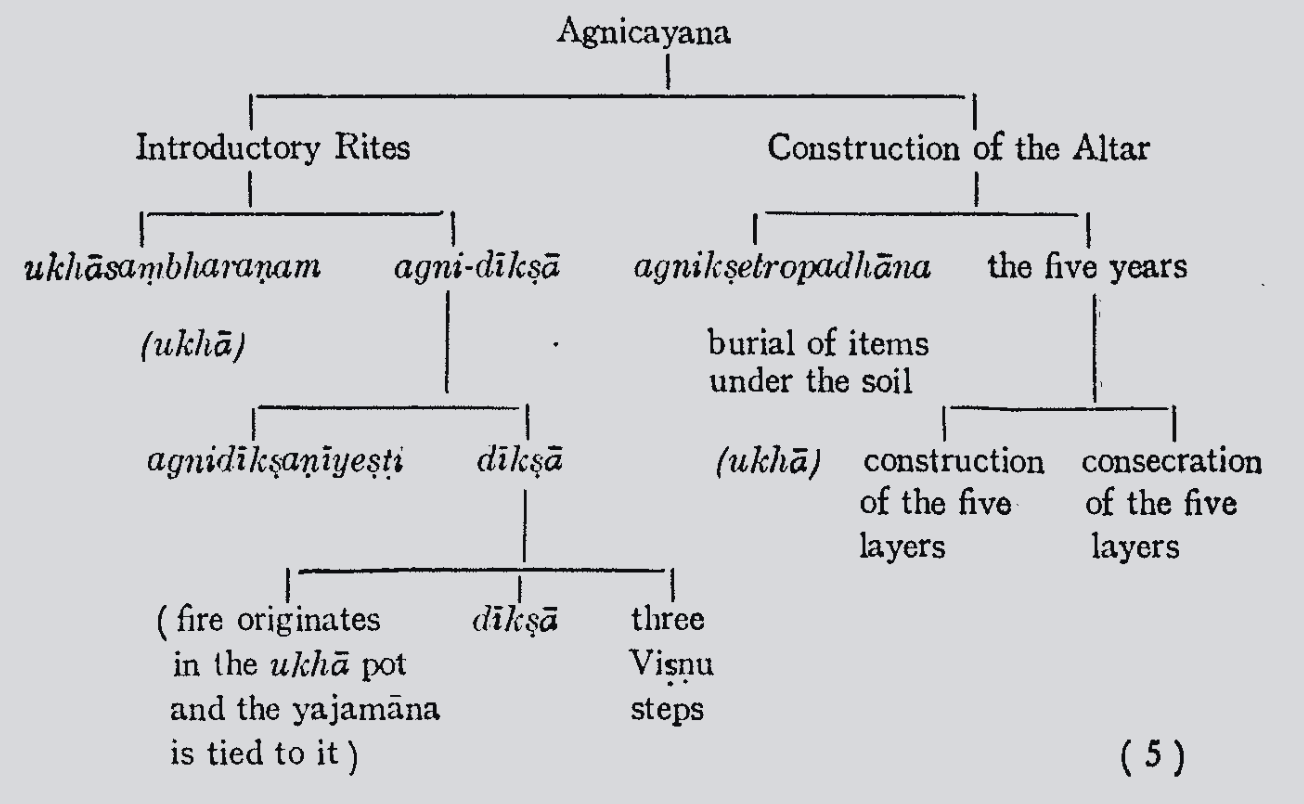
\includegraphics[scale=0.75]{img/staal1984_ritualsyntax.png} 
  \caption{
    Ritual syntax of the Agnicayana, a Vedic ritual.
    While the \textit{ukh\={a}} pot is used in several different rites throughout the ritual, these rites do not occur subsequentially. 
    Rather, the ceremonies involving the \textit{ukh\={a}} pot are center-embedded at different points throughout the ritual. 
    Reproduced from \cite{staal1984ritual}.
  }.\label{fig:staal1984_ritualsyntax}
\end{figure}

I advance Staal's thesis for the evolution of language by offering the practice of mathematics as yet another human activity with center-embedding that derives from ritual.  
By no means is mathematics the only human activity that can serve this role. 
For example, storytelling manifesting as poetry and literature is another. 
Not only does storytelling exhibit recursion via thematic framing and the device of embedding a story inside another story \parencite{minkowski1989janamejayas, niles1979ring},
\cite{minkowski1989janamejayas}'s analysis of the relationship between the ancient Smruti epic \textit{Mah\={a}bh\={a}rata} and Vedic rituals offers strong evidence that the practice of literature originates from ritual. 
It follows that humans' capacity to center-embed in literature also originates from ritual.  
I offer a similar analysis via the practice of mathematics. 
As will be demonstrated, mathematical arguments exhibit center-embedded structure sharing key features to center-embedding in natural langauge. 
Furthermore, the history of mathematics and ritualistic behavior in mathematics research and education indicate the practice of mathematics has ritual roots. 
The identification of mathematics as yet another center-embedding human activity derived from ritual strengthens Staal's claim that the human capacity for center-embedding is adapted specifically for ritual, not language; 
consequently, ritual is the precursor to language. 

\vspace{1.5em} 
The proof of the following claim demonstrates the structure of center-embedding in mathematical arguments. 
\begin{claim} \label{thm:rt2_irrat}
  $\sqrt{2}$ is irrational. 
\end{claim}
\begin{proof}[Proof of Claim \ref{thm:rt2_irrat}]
  \textbf{For contradiction, suppose $\sqrt{2}$ is not irrational}; 
  that is, assume $\sqrt{2}$ is rational.
  Then $\sqrt{2} = \frac{p}{q}$ for some relatively prime positive integers $p$ and $q$ (they have no common divisor). 
  Multiplying both sides by $q$ and squaring, obtain 
  \begin{equation} \label{eq:contr_eq}
    2q^2 = p^2.
  \end{equation}
  Since $p^2$ is an integer multiplied by 2, $p^2$ must be even. 
  But $p^2$ can only be even if $p$ is even; 
  thus, 4 divides $p^2$. 
  Let $p^2 = 4m$ for some integer $m$. 
  Then cancelling 2 from both sides of \eqref{eq:contr_eq} yields 
  $$q^2 = 2m,$$
  so it follows that $q^2$ is even.
  By the same reason as $p^2$, $q^2$ can only be even if $q$ is even. 
  Hence $p$ and $q$ are both even; 
  they are both divisible by 2. 
  This contradicts the assumption that $p$ and $q$ are relatively prime. 
  \textbf{The contradiction shows that $\sqrt{2}$ is irrational.} 
\end{proof}

In this proof, the core argument, which I will call the argument at depth 1, is embedded within the boldfaced statements, 
i.e., the assumption that $\sqrt{2}$ is rational and the conclusion that $\sqrt{2}$ is irrational, which I will call the depth 0 argument.  
This structure is indeed a center-embedding that parallels center-embedding in natural language. 
First, there is a dependency between the opening assumption ($\sqrt{2}$ is rational) and the closing conclusion ($\sqrt{2}$ is irrational);
one does not start a contradiction argument by assuming a statement to be false without deriving a contradiction arising from that false assumption to show that the statement is indeed true. 
Second, there is a dependency between the outer depth 0 statements -- that is, the assumption and conclusion about whether $\sqrt{2}$ is rational -- and the embedded depth 1 argument -- the line of reasoning deriving the contradiction caused by the assumption $\sqrt{2}$ is rational. 
Of course, the argument at depth 1 is entirely dependent on the assumption made at depth 0. 
Less trivial is that the argument at depth 1 must be fully contained within the boundaries of depth 0: 
once $\sqrt{2}$ is taken to be rational at the start of depth 0, this assumption must be held for the entirity of depth 1, and once a contradiction is derived at depth 1 to fulfill the dependency at depth 0, the arguments made in depth 1 become inaccessible to arguments succeeding the conclusion of depth 0 precisely because the conclusion of depth 0 establishes that $\sqrt{2}$ is irrational.  
Third, just like in natural language, it is possible to embed additional layers of mathematical arguments, though for the sake of clarity, high levels of embedding are avoided. 
If I was to suppress brevity and be more complete in my mathematical argument in the proof of Claim \ref{thm:rt2_irrat}, I would have imbedded another layer of argument justifying why $p^2$ is even if and only if $p$ is even, leading to a depth-2 center-embedded mathematical argument whose structure is abstracted in Figure \ref{fig:proof_str}. 
Evidently, center-embedding in mathematical arguments and in natural language follow a parallel set of rules and display similar properties. 

\begin{figure}
  \centering
  \large
  \begin{tabular}[t]{@{}l@{}}
    0: \textit{Assume $\sqrt{2}$ is rational.} \\
    \quad 1: \textit{Let $\sqrt{2} = \frac{p}{q}$ for relatively prime $p$ and $q$ to} \\ 
    \quad \textit{derive the equation $2q^2 = p^2$.} \\
    \qquad 2: \textit{Take $p^2$ to be even} \\
    \qquad 2: \textit{Conclude $p$ is even.} \\
    \quad 1: \textit{Using the fact $p$ is even, show that $q$ is even} \\ 
    \quad  \textit{as well, which contradicts the assumption that} \\ 
    \quad \textit{$p$ and $q$ are relatively prime.} \\
    0: \textit{Conclude $\sqrt{2}$ is irrational.} \\
  \end{tabular}

  \caption{
    A schematic of the mathematical argument presented in the proof of Claim \ref{thm:rt2_irrat}, where an additional argument is provided at depth 2 to show why $p$ is even if $p^2$ is even.
  } \label{fig:proof_str}
\end{figure}

What is notable is not that center-embedding occurs at all in mathematical arguments -- this is to be predicted given the logic inherent in mathematics -- but rather that humans easiliy process center-embedded mathematical arguments online (e.g., during a lecture). 
Indeed, center-embedded arguments far more complicated than the proof of Claim \ref{thm:rt2_irrat} occur several times during a 50-minute lecture for introductory pure math classes. 
Contrast the ease of processing center-embeddeding in a mathematical argument to the difficulty comprehending the following center-embedding in natural language: 
\begin{center}
  \begin{minipage}{0.8\linewidth}
    All told, the Post is now a significantly smaller news organization, and one that many journalists who care deeply about the institution worry will be significantly less ambitious... \footnotemark
  \end{minipage}
\end{center}
\footnotetext{Jeremy Barr, ``Mass layoffs at Washington Post,'' \textit{The Guardian}, February 5, 2026, \url{https://www.theguardian.com/media/2026/feb/05/mass-layoffs-washington-post}. Found by Professor Robert Kluender.} 
Although the sentence above is more readable compared to artificial center-embedded sentences created for experimental purposes, I still find it quite difficult to parse;
on first read, paper and pencil were needed to verify the dependencies. 
The relative ease with which center-embedded mathematical arguments can be understood reemphasizes the unique difficulty humans have processing center-embedded structure in the context of language. 
If the capacity for recursion evolved for the purpose of language, why is it that language is the specific domain where instances of center-embedding are hardest to process?  
Note that, like ritual and literature, there is no obvious mechanic that ameliorates the burden of processing center-embedded mathematical arguments. 
While the logic inherent in math increases the likelihood that center-embedding may occur, humans ultimately deliver mathematical arguments via natural language, not rigorous formal logic;
instead, as \cite{lipton1979social} put it, ``the proof of a theorem is a message," a persuasion that a completely rigorous formal justification exists without actually supplying that formalization. 
With this consideration, I posit that the internal cognitive representation of center-embedded mathematical arguments is similar to to that of center-embedding in ritual and literature, unaffected by the logical nature of math. 
If this is indeed true, then mathematics is yet another human activity where center-embedding, for whatever nontrivial reason, is natural and easy for humans to produce and process, adding credence to Staal's hypothesis that the cognitive systems sufficient for language originates from an older human activity. 

\vspace{1em}
The evidence from mathematics supports the hypothesis of the ritual origin of language because there is strong evidence that math, too, derives from ritual. 
If, like literature, mathematics is indeed another center-embedding human activity derived from ritual, then the hypothesis that the human cognitive system for center-embedding developed for the purposes of ritual gains further credibility. 
First, I offer a historical perspective. 
Admittedly, whether one concludes that math historically derives from ritual may depend on which practices one considers to be math. 
Some contemporary mathematicians may designate set theory, type theory, or category theory as the basis for math. 
Instead, I endorse Fields medalist Richard Borcherds's insight that ``the foundations [of math will] always consist of properties of the natural numbers."% 
\footnote{Richard Borcherds, ``Questions and Answers 1," YouTube, March 5, 2021, \url{https://youtu.be/D87jIKFTYt0?si=uI-Sz0YpHVLPId5Y&t=392}.}
Because the theory of numbers is often realized through geometric properties, I also include geometry as the foundation of math. 

Although Richard Borcherds likely ascends the study of the natural numbers as the foundation of mathematics due to philosophical reasons from relatively recent developments in math, Abraham Seidenberg's studies lend ancient-historic merit to Borcherds's view. 
Taking inspiration from the following Pythagorean number mysticism, \cite{seidenberg1962counting} argues that basic counting systems originate from rituals celebrating religious procession. 
\begin{enumerate}
  \centering
  \item Odd numbers are male 
  \item Ten is a perfect number 
  \item Five is a marriage number 
  \item One is God 
  \item One is both even and odd 
  \item Everything is number,
\end{enumerate}
While the context of religious procession motivates why a ritual may involve counting, Seidenberg makes the key observation that myths are rites manifested in words
\footnote{In his analysis, Seidenberg assumes language as predating counting: 
``The basic things needed for counting are a definite sequence of words and a familiar activity in which they are employed. 
The creation ritual offers us precisely such sequence and activity" \parencite[p. 8]{seidenberg1962counting}.
Though certainly interesting and valuable, accepting or rejecting this assumption is beyond the scope of this essay; 
whether language predates math is inconsequential to establishing the relationship between math and ritual, and therefore unrelated to the objective of identifying ritual as the source of center-embedding.} \label{ft:lang_pred_math}
and therefore independent from speculation, explanation, and history;
as such, the art of counting itself becomes the focus of rites celebrating procession, not the beliefs motivating the need to count.
Seidenberg's analysis of procession rituals parallels \cite{staal1984search}'s thesis that ritual is performed and maintained with regard to structure alone, adding credibility to the designation of ritual as the origin of counting.  
While \cite{seidenberg1962counting} does not name a particular culture as the origin of counting, \cite{seidenberg1961geometry} specifies that the basic art of counting developed into the theory of numbers and geometry in the context of Vedic rituals. 
Seidenberg considers classical mathematical problems such as the Pythagorean theorem, the squaring of a circle, and the duplication of a cube.
Challenging the common attributtion of these problems to ancient Greek mathematics, Seidenberg finds that these problems harken back to the \textit{Sulvasutra}, an ancient Vedic text detailing the geometric construction of sacrifical altars. 
Take, for example, the construction of a falcon altar, where the theological motivation for its creation is that the altar embodies a real falcon enabling the sacrificer to reach the heaven. 
The process explicitly requires the determination of which sum of squares equals another square and converting various shapes into another; 
geometric precision is necessary for the creation of the sacrificial altar.
Mathematically, such constructions are only possible by considering the classical ``Greek" problems, so it follows that these mathematical theories were a central component of Vedic altar rituals. 
In fact, it is more plausible that the Pythagorean theorem, constructing squares from circles and vice versa, duplicating a cube, etc. originated from ritual context and disseminated into a more secular practice, such as Greek mathematics, rather than the other way around: 
considering the characteristics of ritual explored thus far, it seems perfectly plausible that mathematical theory originated from theology, abstracted as mathematical practice became ritualized, and then eventually broke off into ``pure," secular study of mathematical properties alone;
on the other hand, if one posits Vedic ritualists imported secular mathematics, from the Greeks for example, one would have to motivate why these ritualists adopted a technical tool as such an integral part of their ritual. 
Just as \cite{seidenberg1962counting} appeals to ritual's inherent focus on structure to identify ritual as the source of counting, the most fundamental mathematical concept, it seems that the theories of numbers and geometry were further developed in ritual context as well. 

\vspace{1.5em} 
Next, I briefly examine the ritualistic nature of mathematical practices today, both among professional mathematicians and grade school students. 
At first glance, it is curious that professional mathematicians would practice math ritually; 
one would think that, given both their mastery for the subject and their limited time, professional mathematicians (would at least try to) optimize their time to effectively understand and teach mathematics. 
Yet this is blatantly not the case for math seminars. 
Seminars are important to mathematics departments in universities; 
its import can be conveyed via the amount of time professors and graduate students spend organizing and attending the seminars;
many research math professors at UCSD, for example, cancel at least one or two sessions of the classes they teach every quarter in order to attend seminars and conferences at other institutions. 
However, \textit{why} conferences are important is hard to pinpoint. 
As \cite{barany2014chalk} account, even mathematicians within the same subfield of study have ``comparatively little idea of what each other does" and attend seminars to, at best, vaguely follow the arguement and narrative presented by the speaker, let alone understand detailed proofs of theorems. 
Many are ``easily bored and prone to distraction."
Even though minor preparation by reading the speaker's works would greatly improve understandability during the seminar, most attendees do not do so. 
Such behavior suggests that teaching, or even loosely expositioning, mathematics is not the main goal of conducting seminars; 
an email exchange sending the material of interest, an independent reading of that topic, and perhaps brief feedback seems far more effective for the sole goal of teaching and learning math for both the seminar speaker and attendees. 
For some, seminars may be a social oppotunity; 
I propose that for many others, seminar serves a ritual function where mathematicians organize, attend, and speak in seminars just for the practice of doing so. 
Indeed, as a speaker interviewed by Barany and MacKenzie puts it, 
``[Seminars are] a bit like a beehive... collecting nectar and pollen doesn't benefit the specific bee so well, but it's important for the community."  

The ritualistic practice of math is also seen in grade school education. 
In general, there is an abudance of literature in education studies examining ``ritualized" learning, where a curriculum encourages students to learn via a feeling of communual belonging (e.g., social pressure) and meaningless drills rather than active exploration of topics.  
However, given that many students' enduring impression of mathematics is that it is overly abstract or even esoteric, many in the educational sciences have applied the perspective of ritual specifically to math education. 
Such a ``ritual" is aptly demonstrated by \cite{robertson2019exploratory}, who analyze how the compounded difficulty of learning mathematics and receiving schooling in a second language induces ineffective learning behavior amongst grade school students in South Africa. 
In their corpus study of a grade 4 classroom session on fractions, Robertson and Graven conclude that 58\% of the students' responses were chorused while 42\% were individualized. 
Chorused responses often indicate ineffective learning because it occurs as mob behavior; 
rather than demonstrating their own understanding, students simply repeat the answer blurted out by another. 
Meanwhile, even amongst the 42\% of individualized responses, many students couldn't justify why they responded so when further prompted by the teacher. 
Clearly, such a learning model is ineffective, yet the teacher moves on acknowledging the students' poor understanding for the sake of time. 
Thus, this learning setting is ritualized: 
the students' responses during lessons are meaningless because it does not demonstrate any real learning, which makes the entire lesson meaningless because no effective teaching and learning is accomplished;
yet these superficial, meaningless performances of learning and teaching are conducted for the sake of educational structure. 
By no means is this a problem occuring solely in the instruction of math.
As noted previously, ritualized behaviors occur generally in education. 
Similarly, I'm sure seminars in all other academic disciplines have some ritualistic aspect to them. 
However, the ritualization of math seems particularly noteworthy due to both math's historical origins and the abstract structure inherent in mathematics;
thus, ritualistic instinct during mathematical practice may be particularly salient. 

\vspace{1.5em}
In this essay, I exhibited center-embedded structure in mathematical arguments and pointed to the ritual origin of mathematics to support Fritz Staal's hypothesis that recursion, and therefore language, harkens back to ritual. 
As was demonstrated for center-embedding in ritual \parencite{staal1984ritual}, center-embedding in mathematics shares notable features with center-embedding in natural langauge, hinting ritual as the shared origin between mathematical practice and language. 
Other human activities demonstrating recursion were less successful at serving this mean because the claimed occurence of center-embedding in those activities had key differences from center-embedding in langauge. 
Particularly, the relation between toolmaking and language has been extensively studied. 
\cite{stout2009making} suggest the shared neurobiology of toolmaking and language, partly by citing the activation of the Posterior Broca's area during both toolmaking and language syntactic processing.  
\cite{stout2011stone} furthers this idea by highlighting similarities between syntactic recursion in langauge and the action sequence hierarchy of creating stone tools from various points in ancient human history.  
However, generativists have discredited Stout's theory due to the lack of dependency between ``center-embedded" action sequences: 
for example, during toolmaking, it is not necessary that the core of a flake be struck after positioning the core and gripping the hammerstone \parencite{berwick2017why, moro2014response}.  
Whether these discrepencies are truely relevant for the purpose of langauge evolution is to be seen. 
Regardless, center-embedding in math does not suffer from this line of criticism because, as I have shown, a valid center-embedded mathematical argument follows a strict set of rules akin to that of language syntax. 
Furthermore, the ritual origin of mathematics increases the likelihood that there is a nontrivial relationship between center-embedding in ritual, mathematics, and language. 

On its own, mathematics alone is insufficient justification for the claim that language derives from ritual. 
At the moment, there is not enough direct empirical evidence to conclude that the neurobiological basis for ritual gave way to the cognitive system sufficient for language. 
Meanwhile, when considered in isolation, it is not impossible that the shared center-embedding structure in math and language is due to mathematical arguments being parasitic on language, not ritual. 
Yet taking into account center-embedding in literature, music, and other ancient human activities that are more likely to have originated from ritual than language, the hypothesis that the human capacity for center-embedding evolved for the purposes of ritual becomes increasingly convincing. 
Thus, by elucidating the connections between mathematics, ritual, and languge, I wish to motivate the identification of more human activities that may ultimately validate Staal's hypothesis for the evolution of language. 


\newpage
\section*{Acknowledgement}
I used claude.ai to help typeset some of the figures. 
Thank you to Janice Kim for helpful feedback throughout the writing process. 
Thank you to Robert Kluender for the enlightening quarter. 

\printbibliography

\end{document}
